\chapter{Recurrences}
\label{ch:analysis::recurrences}

\begin{cluster}
\label{grp:prmbl:analysis::recurrences::covers}

\begin{preamble}
\label{prmbl:analysis::recurrences::covers}
This chapter covers recurrences  and presents
three methods for solving recurrences: 
the \href{sec:analysis::recurrences::tree-method}{``Tree Method''}
the \href{sec:analysis::recurrences::brick-method}{``Brick Method''}, and
the \href{sec:analysis::recurrences::master-method}{``Substitution Method''}.

\end{preamble}
\end{cluster}


\section{The Basics}
\label{sec:analysis::recurrences::the-basics}

\begin{cluster}
\label{grp:grm:analysis::recurrences::recurrences}

\begin{gram}
\label{grm:analysis::recurrences::recurrences}
  Recurrences are simply recursive functions for which the argument(s) and
  result are numbers. 
  As is normal with recursive functions, recurrences have a recursive
  case along with one or more base cases.
  Although recurrences have many applications, in this book we mostly use
  them to represent the cost of algorithms, and in particular their
  work and span.
  They are typically derived directly from recursive algorithms by
  abstracting the arguments of the algorithm based on their sizes, and
  using the cost model described in \chref{analysis::models}.
  Although the recurrence is itself a function similar to the
  algorithm it abstracts, the goal is not to run it, but instead the
  goal is to determine a closed form solution to it using other
  methods.
  Often we satisfy ourselves with finding a closed form that specifies an
  upper or lower bound on the function, or even just an asymptotic
  bound.

\end{gram}
\end{cluster}

\begin{cluster}
\label{grp:xmpl:analysis::recurrences::fibonacci}

\begin{example}[Fibonacci]
\label{xmpl:analysis::recurrences::fibonacci}
Here is a recurrence written in \PML{} that you should recognize:
\[
\begin{array}{ll}
F(n) =&\cd{case}~n~\cd{of}
\\ 
& ~~~~0~~\cdra~0
\\
& ~~|~1~~\cdra~1
\\
& ~~|~\_~~\cdra~F(n-1) + F(n-2)~~.
\end{array}
\]
It has an exact closed form solution:
 \[F(n) = \frac{\varphi^n - (1 - \varphi)^n}{\sqrt{5}}~,\]
where $\varphi = \frac{1 + \sqrt{5}}{2}$ is the golden ratio.
We can write this in asymptotic notation as \[F(n) =
\Theta(\varphi^n) \]
since the first term dominates asymptotically.

\end{example}
\end{cluster}

\begin{cluster}
\label{grp:ex:analysis::recurrences::mergesort}

\begin{example}[Mergesort Recurrence]
\label{ex:analysis::recurrences::mergesort} 
Assuming that the input length is a power of $2$, we can write the code for parallel mergesort algorithm as follows.
\[
\begin{array}{l}
\cdvar{msort}(A) = 
\\
~~~~\cd{if}~|A| \leq 1~\cd{then}~A 
\\
~~~~\cd{else}
\\
~~~~~~~\cd{let}~(L,R) 
  =~\cdvar{msort}(A[0 \dots |A|/2])~||~\cdvar{msort}(A[|A|/2 \dots|A|]) 
\\
~~~~~~~\cd{in}~\cdvar{merge}(L,R)~\cd{end}
\end{array}
\]
By abstracting based on the length of $A$, and using the cost model
described in \chref{analysis::models}, we can write a recurrence for the work of mergesort as:
\[
\begin{array}{l}
W_{\cdvar{msort}}(n) = 
\\
~~~~\cd{if}~n \leq 1~\cd{then}~c_1
\\
~~~~\cd{else}
\\
~~~~~~~\cd{let}~(W_L,W_R) 
  =~(W_{\cdvar{msort}}(n/2), W_{\cdvar{msort}}(n/2)) 
\\
~~~~~~~\cd{in}~W_L + W_R + W_{\cdvar{merge}}(n)+ c_2~\cd{end}
\end{array}
\]
where the $c_i$ are constants.    Assuming 
$W_{\cdvar{merge}}(n) = c_3 n + c_4$ this can be simplified to
\[
\begin{array}{ll}
W_{\cdvar{msort}}(n) = &\cd{if}~n \leq 1~\cd{then}~c_1
\\
&\cd{else}~2 W_{\cdvar{msort}}(n/2) + c_3 n + c_5
\end{array}
\]
where $c_5 = c_2 + c_4$.    We will show in this chapter that this
recurrence solves to
\[W_{\cdvar{msort}}(n) = O(n \lg n) \]
using all three of our methods.

\end{example}
\end{cluster}


\section{Some conventions}
\label{sec:analysis::recurrences::some-conventions}

\begin{cluster}
\label{grp:grm:analysis::recurrences::reduce}

\begin{gram}
\label{grm:analysis::recurrences::reduce}
To reduce notation we use several conventions when writing recurrences.

\end{gram}
\end{cluster}

\begin{cluster}
\label{grp:grm:analysis::recurrences::syntax}

\begin{gram}[Syntax]
\label{grm:analysis::recurrences::syntax}
We typically write recurrences as mathematical relations of the form
\[
W_f(n) = \left\{
\begin{array}{lll}
c_1 & \mbox{base case 1} 
\\
c_2 & \mbox{base case 2} 
\\
\cdots& \cdots
\\
\mbox{recursive definition}  &  \mbox{otherwise}.
\end{array}
\right. 
\]

\end{gram}
\end{cluster}

\begin{cluster}
\label{grp:grm:analysis::recurrences::dropping-the-subscript}

\begin{gram}[Dropping the subscript]
\label{grm:analysis::recurrences::dropping-the-subscript}
We often drop the subscript on the cost $W$ or $S$ (span) when obvious from the context.

\end{gram}
\end{cluster}

\begin{cluster}
\label{grp:grm:analysis::recurrences::base-case}

\begin{gram}[Base case]
\label{grm:analysis::recurrences::base-case}
Often  base cases are trivial---i.e., some constant if $n
\leq 1$.  In such cases, we usually leave them out.

\end{gram}
\end{cluster}

\begin{cluster}
\label{grp:grm:analysis::recurrences::big-o-inside-a-recurrence}

\begin{gram}[Big-O inside a recurrence]
\label{grm:analysis::recurrences::big-o-inside-a-recurrence}
Technically using big-O notation in a recurrence as in:
\[ 
W(n) = 2 W(n/2) + O(n) 
\]
is not well defined.   
This is because $2 W(n/2) + O(n)$ indicates a
set of functions, not a single function.    
In this book when we use
$O(f(n))$ in a recurrences it is meant as shorthand for $c_1 f(n) +
c_2$, for some constants $c_1$ and $c_2$. 
Furthermore, when solving the recurrence the $O(f(n))$ should
always be replaced by $c_1 f(n) + c_2$.

\end{gram}
\end{cluster}

\begin{cluster}
\label{grp:grm:analysis::recurrences::inequality}

\begin{gram}[Inequality]
\label{grm:analysis::recurrences::inequality}
Because we are mostly concerned with upper bounds,  we can be  sloppy and 
add (positive) constants on the right-hand side of an equation.
In such cases, we typically use an inequality, as in
\[ 
W(n) \leq 2 W(n/2) + n.
\]

\end{gram}
\end{cluster}

\begin{cluster}
\label{grp:grm:analysis::recurrences::input-size-inprecision}

\begin{gram}[Input size inprecision]
\label{grm:analysis::recurrences::input-size-inprecision}
A technical issue concerns rounding of input sizes.
Going back to the \href{ex:analysis::recurrences::mergesort}{mergesort example}, note that we assumed that the size
of the input to merge sort, $n$, is a power of $2$.
If we did not make this assumption, i.e., for general $n$, 
we would partition the input into two parts, whose sizes may differ by up to one element.
In such a case, we could write the work recurrence as 
\[
W(n) = \left\{
\begin{array}{ll}
O(1) & \mbox{if} ~ n \le 1
\\
W(\lceil n/2 \rceil) + W(\lfloor n/2 \rfloor) + O(n) &  \mbox{otherwise}.
\end{array}
\right.
\]

When working with recurrences, we typically ignore floors and ceiling
because they change the size of the input by at most one, which
does not usually affect the closed form by more than a constant
factor.

\end{gram}
\end{cluster}

\begin{cluster}
\label{grp:xmpl:analysis::recurrences::mergesort-recurrence-revisited}

\begin{example}[Mergesort recurrence revisited]
\label{xmpl:analysis::recurrences::mergesort-recurrence-revisited}
Using our conventions we can write our recurrence for the work of
mergesort as:
\[W(n) \leq 2W(n/2) + O(n)~.\]
However, when solving it is best to write it as:
\[
W(n) \leq \left\{
\begin{array}{lll}
c_b & \mbox{if}~n \leq 1
\\
2W(n/2) + c_1 n + c_2 & \mbox{otherwise} ~.
\end{array}
\right. 
\]
Assuming $\cdvar{merge}$ has logarithmic span, we can similarly write
a recurrence for the span of the parallel mergesort as:
\[S(n) \leq S(n/2) + O(\lg n)~.\]

\end{example}
\end{cluster}


\section{The Tree Method}
\label{sec:analysis::recurrences::tree-method}

\begin{cluster}
\label{grp:def:analysis::recurrences::tree-method}

\begin{definition}[Tree Method]
\label{def:analysis::recurrences::tree-method}
The~\defn{tree method} is a technique for solving recurrences.
Given a recurrence, the idea is to derive a closed form solution of
the recurrence by first unfolding the recurrence as a tree and then
deriving a bound by considering the cost at each level of the tree.
To apply the technique, we start by replacing the asymptotic notations
in the recurrence, if any.
We then draw a tree where each recurrence instance is represented by a
subtree and the root is annotated with the cost that occurs at this
level, that is beside the recurring costs. 

After we determine the tree, we ask several questions.
\begin{itemize}
\item How many levels are there in the tree?
\item What is the problem size on level $i$?
\item What is the cost of each node on level $i$?
\item How many nodes are there on level $i$?
\item What is the total cost across the level $i$?
\end{itemize}

Based on the answers to these questions, we can write the cost as a
sum and calculate it.

\end{definition}
\end{cluster}

\begin{cluster}
\label{grp:tch:analysis::recurrences::todo}

\begin{teachnote}
\label{tch:analysis::recurrences::todo}
TODO: we can place a ref to a cross chapter atom in the atom below

\end{teachnote}
\end{cluster}

\begin{cluster}
\label{grp:xmpl:analysis::recurrences::consider}

\begin{example}
\label{xmpl:analysis::recurrences::consider}
Consider the recurrence
$$
W(n) = 2W(n/2) + O(n).
$$
By the definition of asymptotic complexity, we
can establish that
\begin{eqnarray*}
  W(n) &\leq& 2W(n/2) + c_1\cdot n + c_2,
\end{eqnarray*}
where $c_1$ and $c_2$ are constants.  

We now draw a tree to represent the recursion. Since there are two
recursive calls, the tree is a binary tree, whose input is half the
size of the size of the parent node.
We then annotate each node in the tree with its cost noting that if
the problem has size~$m$, then the cost, excluding that of the
recursive calls, is at most~$c_1 \cdot m + c_2$.  

The drawing below illustrates the resulting tree; each level is
annotated with the problem size (left) and the cost at that level
(right).

\begin{center}
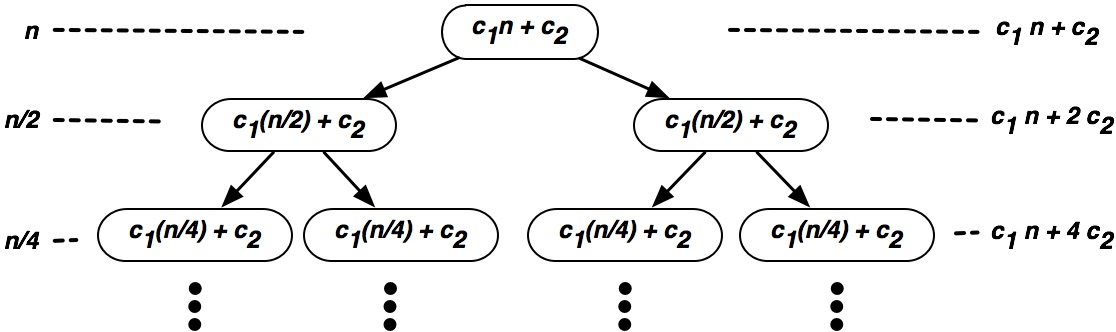
\includegraphics[width=4.5in]{./analysis/media-recurrences/recurtree1.jpg}
\end{center}

We observe that:
\begin{itemize}
\item  level $i$ (the root is level $i=0$) contains $2^i$
nodes, 
\item a node at level $i$ costs at most $c_1 (n/2^i) + c_2$.
\end{itemize}
Thus, the total cost on level $i$ is at most
\begin{eqnarray*}
2^i \cdot \left(c_1 \frac{n}{2^i} + c_2\right) &=& c_1 \cdot n + 2^i \cdot c_2.
\end{eqnarray*}

Because we keep halving the input size, the number of levels $i \le
\lg n$.  Hence, we have
\begin{eqnarray*}
  W(n) &\leq& \sum_{i=0}^{\lg n} \left(c_1 \cdot n + 2^i \cdot c_2\right) \\
  &=& c_1 n (1+\lg n)+ c_2(n +\tfrac{n}{2} + \tfrac{n}{4} + \dots + 1)\\
  &=& c_1 n (1+\lg n)+ c_2(2n - 1)\\
  &\in& O(n\lg n),
\end{eqnarray*}
where in the second to last step, we apply the fact that for $a > 1$,
\[ \begin{equation*}
1 + a + \dots + a^{n} = \frac{a^{n+1} - 1}{a-1} \leq a^{n+1}.
\end{equation*} \]

\end{example}
\end{cluster}


\section{The Brick Method}
\label{sec:analysis::recurrences::brick-method}

\begin{cluster}
\label{grp:grm:analysis::recurrences::brick}

\begin{gram}
\label{grm:analysis::recurrences::brick}
  The~\defn{brick method} is a special case of the tree method, aimed
  at recurrences that grow or decay geometrically across levels of the
  recursion tree.
  A sequence of numbers has \defn{geometric growth} if it grows by at
  least a constant factor ($> 1$) from element to element, and has \defn{geometric decay} if it decreases by at least a constant
  factor.  
  The beauty of a geometric sequence is that its sum is
  bounded by a constant times the last element (for geometric growth), or
  the first element (for geometric decay).

\end{gram}
\end{cluster}

\begin{flex}
\label{grp:xrcs:analysis::recurrences::sums-of-geometric-series}

\begin{exercise}[Sums of geometric series.]
\label{xrcs:analysis::recurrences::sums-of-geometric-series}
  Consider the sum of the sequence $S = \langle 1, \alpha, \alpha^2,
  \ldots, \alpha^n \rangle$.   Show that
\begin{enumerate}
\item
 for $\alpha > 1$ (geometric growth), the sum of $S$ is at most
  $\left(\frac{\alpha}{\alpha -1}\right) \cdot \alpha^n$, and 
\item
for $\alpha < 1$ (geometric decay), the
  sum of $S$ is at most  $\left(\frac{1}{1 - \alpha}\right) \cdot 1$.
\end{enumerate}
Hint: for the first let $s$ be the sum, and consider $\alpha s - s$, cancelling
terms as needed.

\end{exercise}

\begin{solution}
\label{sol:analysis::recurrences::solve}
Let
\[s = \sum_{i=0}^n \alpha^i~.\]
To solve the first case we use
\[ 
\begin{array}{lcl}
\alpha s - s & = & \left(\alpha \sum_{i=0}^n \alpha^i\right) -
                   \sum_{i=0}^n \alpha^i\\
                  & = & \left(\sum_{i=0}^n \alpha^{i+1}\right) -
                        \sum_{i=0}^n \alpha^i\\
                  & = & \alpha^{n+1} - 1\\
                  & < & \alpha^{n+1} ~.
\end{array}
\]
Now by dividing through by $\alpha - 1$ we get
\[ s < \frac{\alpha^{n+1}}{\alpha-1} = \left(\frac{\alpha}{\alpha-1}\right)
  \cdot \alpha^n~, \]
which is we wanted to show.

The second case is similar but using $s - \alpha s$.

\end{solution}
\end{flex}

\begin{cluster}
\label{grp:grm:analysis::recurrences::tree}

\begin{gram}
\label{grm:analysis::recurrences::tree}
  In the tree method, if the costs grow or decay geometrically across
  levels (often the case), then for analyzing asymptotic costs we need only consider the
  cost of the root (decay) , or the total cost of the leaves (growth).
  If there is no geometric growth or decay then it often suffices to
  calculate the cost of the worst level (often either the root or
  leaves) and multiply it by the number of levels.
  This leads to three cases which we refer to as root dominated, leaf 
  dominated and balanced.   
  Conveniently, to distinguish these three cases 
  we need only consider the cost of each node in the 
  tree and how it relates to the cost of its children.

\end{gram}
\end{cluster}

\begin{flex}
\label{grp:def:analysis::brick-method}

\begin{definition}[Brick Method]
\label{def:analysis::brick-method}
Consider each node $v$ of the recursion tree, and let $N(v)$ denote  
its input size, $C(v)$ denote its cost, and $D(v)$ denote the set of
its children.   There exists constants $a \geq 1$ (base size), $\alpha
> 1$ (grown/decay rate) such that:

\begin{description}

\item[Root Dominated]
For all nodes $v$ such that $N(v) > a$,
\[C(v) \geq \alpha \sum_{u \in D(v)} C(u),\]
i.e., the cost of the parent is at least a
constant factor greater than the sum of the 
costs of the children.  In this case, the total cost is dominated by
the root, and is upper bounded 
by $\frac{\alpha}{\alpha - 1}$ times the cost of the root. 

\item[Leaves Dominated]
For all $v$ such that $N(v) > a$, 
\[C(v) \leq \frac{1}{\alpha} \sum_{u \in D(v)} C(u),\]
i.e., the cost of the parent is at least a
constant factor less than the sum of the costs of the 
children.   In this case,
the total cost is dominated by the cost of the leaves, and is upper bounded by $\frac{\alpha}{\alpha - 1}$ times the
sum of the cost of the leaves.
Most often all leaves have constant cost so we just have to count the
number of leaves.

\item[Balanced]
When neither of the two above cases is true.     In this case the cost
is upper bounded by the number of levels times the maximum cost of a
level.
\end{description}

\end{definition}

\begin{proof}
\label{prf:analysis::recurrences::consider}
  We first consider the root dominated case.  For this case if the
  root has cost $C(r)$, level $i$ (the root is level $0$) will have
  total cost at most $(1/\alpha)^i C(r)$.  
  This is because the cost of the children of every node on a level
  decrease by at least a factor of $\alpha$ to the next level.  
  The total cost is therefore upper bounded by
  \[ \sum_{i=0}^{\infty} \left(\frac{1}{\alpha}\right)^i C(r).   \]
  This is a decaying geometric sequence and therefore is upper bounded
  by $\frac{\alpha}{\alpha - 1} C(r)$, as claimed.

  For the leaf dominated case, if all leaves are on the same level and
  have the same cost, we can make a
  similar argument as above but in the other direction---i.e. the
  levels increase geometrically down to the leaves.    The cost is
  therefore dominated by the leaf level.
  In general, however, not all leaves are at the same level.

  For the general leaf-dominated case, let
  $L$ be the set of leaves.
  Consider the cost $C(l)$ for $l \in L$, and account a charge of
  $(1/\alpha)^i C(l)$ to its $i$-th ancestor in the tree (its parent
  is its first ancestor).
  Adding up the contributions from every leaf to the internal nodes of
  the tree gives the maximum possible cost for all internal nodes.
  This is because for this charging every internal node will have a
  cost that is exactly $(1/\alpha)$ the sum of the cost of the
  children, and this is the most each node can have by our assumption of
  leaf-dominated recurrences.
  Now summing the contributions across leaves, including the cost of
  the leaves themselves ($i = 0$), we have as an upper bound on the
  total cost across the tree:
  \[\sum_{l \in L} \sum_{i=0}^{\infty}  \left(\frac{1}{\alpha}\right)^i C(l)~. \]
  This is a sum of sums of decaying geometric sequences, giving an
  upper bound on the total cost
  across all nodes of 
  $\frac{\alpha}{\alpha -1} \sum_{l \in L} C(l)$, as claimed.

  The balanced case follows directly from the fact that the total cost
  is the sum of the cost of the levels, and hence at most the number
  of levels times the level with maximum cost.

\end{proof}
\end{flex}

\begin{cluster}
\label{grp:rmrk:analysis::recurrences::term}

\begin{remark}
\label{rmrk:analysis::recurrences::term}
  The term ``brick'' comes from thinking of each node of the tree as a 
  brick and the width of a brick being its cost.  The bricks can be
  thought of as being stacked up  by level.    A recurrence is leaf dominated if the pile of bricks 
  gets narrower as you go up to the root.  It is root dominated if it 
  gets wider going up to the root.  It is balanced 
  if it stays about the same width. 

\end{remark}
\end{cluster}

\begin{cluster}
\label{grp:xmpl:analysis::recurrences::root-dominated}

\begin{example}[Root dominated]
\label{xmpl:analysis::recurrences::root-dominated}
Lets consider the recurrence 
\[W(n) = 2 W(n/2) + n^2.\]
For a node in the recursion tree of size $n$ we have that the cost of
the node is $n^2$ and the sum of the cost of its children is
$(n/2)^2 + (n/2)^2 = n^2/2$.  In this case the cost has
\textbf{decreased} by a factor of two going down the tree, and hence
the recurrence is root dominated.  Therefore for asymptotic analysis
we need only consider the cost of the root, and we have that
$W(n) = O(n^2)$.

\end{example}
\end{cluster}

\begin{cluster}
\label{grp:grm:analysis::recurrences::leaf}

\begin{gram}
\label{grm:analysis::recurrences::leaf}
  In the leaf dominated case the cost is proportional to the number of
  leaves, but we have to calculate how many leaves there are.  In the common case that all leaves are at the 
  same level (i.e. all recursive calls are the same size), then it is 
  relatively easy.  In particular, one can calculate the number of 
  recursive calls at each level, and take it to the power of the 
  depth of the tree, i.e., $(\mbox{branching factor})^{\mbox{depth}}$.

\end{gram}
\end{cluster}

\begin{cluster}
\label{grp:xmpl:analysis::recurrences::leaf-dominated}

\begin{example}[Leaf dominated]
\label{xmpl:analysis::recurrences::leaf-dominated}
Lets consider the recurrence 
\[
W(n) = 2W(n/2) + \sqrt{n}~.
\]
For a node of size $n$ we have that the cost of the node is $\sqrt{n}$ and 
the sum of the cost of its two children is $\sqrt{n/2} + \sqrt{n/2} =
\sqrt{2} \sqrt{n}$. 
In this case the cost has \textbf{increased} by a factor of $\sqrt{2}$ going down the 
tree, and hence the recurrence is leaf dominated.     
Each leaf corresponds to the base case, which has cost $1$.

Now we need to determine how many leaves there are. 
Since each recursive call halves the input size, the depth of
recursion is going to be $\lg n$ (the number of times one needs to
half $n$ before getting to size $1$).   Now on each level the recursion is
making two recursive calls, so the number of leaves will be $2^{\lg n}
= n$.    We therefore have that $W(n) = O(n)$.

\end{example}
\end{cluster}

\begin{cluster}
\label{grp:xmpl:analysis::recurrences::balanced}

\begin{example}[Balanced]
\label{xmpl:analysis::recurrences::balanced}
Lets consider the same recurrence we considered for the tree method, i.e.,
\[W(n) = 2 W(n/2) + c_1 n + c_2.\]
For all nodes we have that the cost of the node is $c_1 n + c_2$ and
the sum of the cost of the two children is $(c_1 n/2 + c_2) + (c_1 n/2
+ c_2) = c_1 n + 2 c_2$.    In this case
the cost is about the same for the parent and children, and certainly not growing or decaying
geometrically.   It is therefore a balanced recurrence.    The maximum
cost of any level is upper bounded by $(c_1 + c_2) n$, since there are
at most $n$ total elements across any level (for the $c_1 n$ term) and
at most $n$ nodes (for the $c_2 n$ term).
There are $1 + \lg n$ levels, so the total cost is upper bounded
by $(c_1 + c_2) n (1 + \lg n)$.   This is slightly larger than our
earlier bound of $c_1  n \lg n + c_2 (2n - 1)$, but it makes no
difference asymptotically---they are both $O(n \lg n)$.

\end{example}
\end{cluster}

\begin{cluster}
\label{grp:rmrk:analysis::recurrences::used}

\begin{remark}
\label{rmrk:analysis::recurrences::used}
  Once you are used to using the brick method, solving recurrences can 
  often be done very quickly.   Furthermore the brick method can give a 
  strong intuition of what part of the program dominates the
  cost---either the root or the leaves (or both if balanced).    This
  can help a programmer decide how to best optimize the performance of
  recursive code.    If it is leaf
  dominated then it is important to optimize the base case, while if
  it is root dominated it is important to optimize the calls to other
  functions used in conjunction with the recursive calls.   If it is
  balanced, then, unfortunately, both need to be optimized.

\end{remark}
\end{cluster}

\begin{flex}
\label{grp:xrcs:analysis::recurrences::recurrences}

\begin{exercise}
\label{xrcs:analysis::recurrences::recurrences}
For each of the following recurrences state whether it is leaf
dominated, root dominated or balanced, and then solve the recurrence
\[
\begin{array}{lcl}
W(n) & = & 3 W(n/2) + n \\
W(n) & = & 2 W(n/3) + n \\
W(n) & = & 3 W(n/3) + n \\
W(n) & = & W(n - 1) + n \\
W(n) & = & \sqrt{n} W(\sqrt{n}) + n^2 \\
W(n) & = & W(\sqrt{n}) + W(n/2) + n \\
\end{array}
\]

\end{exercise}

\begin{solution}
\label{sol:analysis::recurrences::recurrence}
The recurrence $W(n) = 3 W(n/2) + n$  is leaf dominated since $n \leq
3(n/2) = \frac{3}{2}n$.  It has $3^{\lg n} = n^{\lg 3}$ leaves so $W(n) = O(n^{\lg 
  3})$.

The recurrence $W(n) = 2 W(n/3) + n$  is root dominated since $n \geq 
2(n/3) = \frac{2}{3} n.$ 
Therefore $W(n) = O(n)$, i.e., the cost of 
the root.

The recurrence $W(n) = 3 W(n/3) + n$  is balanced since $n = 3(n/3)$.
The depth of recursion is $\log_3 n$, so the overall cost is
$n$ per level for $\log_3 n$ levels, which gives $W(n) = O(n \log n)$.

The recurrence $W(n) = W(n - 1) + n$  is balanced since each level
only decreases by $1$ instead of by a constant fraction.    The
largest level is $n$ (at the root) and there are $n$ levels, which
gives $W(n) = O(n \cdot n) = O(n^2)$.

The recurrence $W(n) = \sqrt{n} W(\sqrt{n}) + n^2$  is root dominated
since $n^2 \geq \sqrt{n} \cdot \left(\sqrt{n}\right)^2 = n^{3/2}$.   In
  this case the decay is even faster than geometric.    Certainly for
  any $n \geq 2$, it satisfies our root dominated condition for
  $\alpha = \sqrt{2}$.
Therefore $W(n) = O(n^2)$.

  The recurrence $W(n) = W(\sqrt{n}) + W(n/2) + n$ is root dominated
  since for $n > 16$, $n \geq \frac{4}{3} (\sqrt{n} + n/2)$.  Note
  that here we are using the property that a leaf can be any problem
  size greater than some constant $a$.  Therefore $W(n) = O(n)$, i.e.,
  the cost of the root.

\end{solution}
\end{flex}

\begin{cluster}
\label{grp:grm:analysis::recurrences::advanced}

\begin{gram}[Advanced]
\label{grm:analysis::recurrences::advanced}
  In some leaf-dominated recurrences 
 not all leaves are at the same level.    An example is
  $W(n) = W(n/2) + W(n/3) + 1$.
  Let $L(n)$ be the number of leaves as a function of $n$.  We can
  solve for $L(n)$ using yet another recurrence.  In particular the
  number of leaves for an internal node is simply the sum of the
  number of leaves of each of its children.  In the example this will
  give the recurrence $L(n) = L(n/2) + L(n/3)$.  Hence, we need to
  find a function $L(n)$ that satisfies this equation.  If we guess
  that it has the form $L(n) = n^{\beta}$ for some $\beta$, we can
  plug it into the equation and try to solve for $\beta$:
\[
\begin{array}{lcl}
n^{\beta} & =  &\left(\frac{n}{2}\right)^{\beta} +
                         \left(\frac{n}{3}\right)^{\beta}\\
             & =  &n^{\beta}\left(\left(\frac{1}{2}\right)^{\beta} +
                    \left(\frac{1}{3}\right)^{\beta}\right)
\end{array}
\]
Now dividing through by $n^{\beta}$ gives 
\[ \left(\frac{1}{2}\right)^{\beta} + \left(\frac{1}{3}\right)^{\beta}
= 1~.\]
This gives $\beta \approx .788$ (actually a tiny bit less).   Hence $L(n) < n^{.788}$, and
because the original recurrence is leaf dominated:
$W(n) \in O(n^{.788})$.

This idea of guessing a form of a solution and solving for it is key
in our next method for solving recurrences, the substitution method.

\end{gram}
\end{cluster}


\section{Substitution Method}
\label{sec:analysis::recurrences::substitution-method}

\begin{cluster}
\label{grp:grm:analysis::recurrences::method}

\begin{gram}
\label{grm:analysis::recurrences::method}
The tree method can be used to find the closed form solution to many
recurrences but in some cases, we need a more powerful techniques that
allows us to make a guess and then verify our guess via mathematical induction.
The substitution method allows us to do that exactly.

\end{gram}
\end{cluster}

\begin{cluster}
\label{grp:imp:analysis::recurrences::technique}

\begin{important}
\label{imp:analysis::recurrences::technique}
This technique can be tricky to use: it is easy to start on the wrong
foot with a poor guess and then derive an incorrect proof, by for example,
making a small mistake.
To minimize errors, you can follow the following tips:
\begin{enumerate}
\item Spell out the constants---do not use asymptotic notation such as
  big-$O$.  The problem with asymptotic notation is that it makes it
  super easy to overlook constant factors, which need to be carefully
  accounted for.

\item Be careful that the induction goes in the right direction.

\item Add additional lower-order terms, if necessary, to make the
  induction work.
\end{enumerate}

\end{important}
\end{cluster}

\begin{cluster}
\label{grp:xmpl:analysis::recurrences::recurrence}

\begin{example}
\label{xmpl:analysis::recurrences::recurrence}
Consider the recurrence
$$
W(n) = 2W(n/2) + O(n).
$$
By the definition of asymptotic complexity, we
can establish that
\begin{eqnarray*}
  W(n) &\leq& 2W(n/2) + c_1\cdot n + c_2,
\end{eqnarray*}
where $c_1$ and $c_2$ are constants.  



We will prove the following theorem using strong induction on $n$.


\textbf{Theorem.}
  Let a constant $k > 0$ be given.  If $W(n) \leq 2 W(n/2) + k \cdot n$ for $n >
  1$ and $W(n) \leq k$ for $n \leq 1$, then we can find constants $\kappa_1$ and
  $\kappa_2$ such that \[ W(n) \;\leq\; \kappa_1 \cdot n \lg n + \kappa_2.\]

\textbf{Proof.}
  Let $\kappa_1 = 2k$ and $\kappa_2 = k$.  For the base case ($n=1$), we check
  that $W(1) \leq k \leq \kappa_2$.  For the inductive step ($n>1$), we assume that
  \[
  W(n/2) \leq \kappa_1 \cdot \tfrac{n}2 \lg (\tfrac{n}2) + \kappa_2,
  \]
  And we'll show that $W(n) \leq \kappa_1 \cdot n \lg n + \kappa_2$.  To show
  this, we substitute an upper bound for $W(n/2)$ from our assumption into the
  recurrence, yielding
  \[ \begin{align*}
    W(n) \;&\leq\; 2W(n/2) + k \cdot n  \\
    \;&\leq\; 2(\kappa_1 \cdot \tfrac{n}2 \lg (\tfrac{n}2) + \kappa_2) + k \cdot n\\
    \;&=\; \kappa_1 n (\lg n - 1) + 2 \kappa_2 + k \cdot n\\
    \;&=\; \kappa_1 n \lg n + \kappa_2 + (k \cdot n + \kappa_2 - \kappa_1 \cdot n)\\
    \;&\leq\; \kappa_1 n \lg n + \kappa_2,
  \end{align*} \]
  where the final step follows because $k \cdot n + \kappa_2 - \kappa_1 \cdot n \leq
  0$ as long as $n > 1$.

\end{example}
\end{cluster}

\begin{cluster}
\label{grp:grm:analysis::recurrences::variants}

\begin{gram}
\label{grm:analysis::recurrences::variants}
Variants of the recurrence considered in our last example arise
commonly in algorithms.  Next, we establish a theorem that shows that
the same bound holds for a more general class of recurrences. 

\end{gram}
\end{cluster}

\begin{flex}
\label{grp:thm:analysis::recurrences::linear-plus}

\begin{theorem}[Superlinear Recurrence]
\label{thm:analysis::recurrences::linear-plus}
Let $\vareps > 0$ be a
constant and consider  the recurrence
\[ \begin{align*}
  W(n) & = 2W(n/2) + k\cdot n^{1+\vareps}.
\end{align*} \]

    If $W(n) \leq 2 W(n/2) + k \cdot n^{1+\vareps}$ for $n > 1$ and $W(n) \leq k$ for $n \leq
  1$, then for some constant $\kappa$, \[ W(n) \;\leq\;
  \kappa \cdot n^{1+\vareps}. \]

\end{theorem}

\begin{proof}
\label{prf:analysis::recurrences::inductive}
  Let $\kappa = \frac1{1-1/2^{\vareps}} \cdot k$. The base case is easy: $W(1) =
  k \leq \kappa_1$ as $\frac1{1 - 1/2^{\vareps}} \geq 1$.  For the inductive
  step, we substitute the inductive hypothesis into the recurrence and obtain
  \begin{eqnarray*}
    W(n) &\leq& 2W(n/2) + k \cdot n^{1+\vareps}\\
    &\leq& 2 \kappa\left(\frac{n}2 \right)^{1+\vareps} + k \cdot n^{1+\vareps}\\
    &=& \kappa \cdot n^{1+\vareps} + \left(2 \kappa\left(\frac{n}2 \right)^{1+\vareps} +
      k \cdot n^{1+\vareps} - \kappa \cdot n^{1+\vareps}\right)\\
    &\leq& \kappa \cdot n^{1+\vareps},
  \end{eqnarray*}
  where in the final step, we use the fact  that for any $\delta > 1$:

  \begin{eqnarray*}
    2 \kappa\left(\frac{n}2 \right)^{\delta} +
    k \cdot n^{\delta} - \kappa \cdot n^{\delta}
    &=& \kappa \cdot 2^{-\vareps} \cdot n^{\delta}  +
    k \cdot n^{\delta} - \kappa \cdot n^{\delta} \\
    &=& \kappa \cdot 2^{-\vareps} \cdot n^{\delta}  +
    (1 - 2^{-\vareps})\kappa\cdot n^{\delta} - \kappa \cdot n^{\delta} \\
    &\leq& 0.
  \end{eqnarray*}


An alternative way to prove the same theorem is to use the tree method
and evaluate the sum directly. The recursion tree here has depth $\lg
n$ and at level $i$ (again, the root is at level $0$), we have $2^i$
nodes, each costing $k\cdot (n/2^i)^{1+\vareps}$.  Thus, the total
cost is
  \begin{eqnarray*}
    \sum_{i=0}^{\lg n} k\cdot 2^i \cdot \pparen{\frac{n}{2^i}}^{1+\vareps}
    &=&  k\cdot n^{1+\vareps} \cdot \sum_{i=0}^{\lg n} 2^{-i\cdot\vareps} \\
    &\leq& k\cdot n^{1+\vareps} \cdot \sum_{i=0}^{\infty} 2^{-i\cdot\vareps}.
  \end{eqnarray*}
  But the infinite sum $\sum_{i=0}^{\infty} 2^{-i\cdot\vareps}$ is at most
  $\frac1{1 - 1/2^{\vareps}}$. Hence, we conclude $W(n) \in O(n^{1+\vareps})$.

\end{proof}
\end{flex}


\section{Master Method}
\label{sec:analysis::recurrences::master-method}

\begin{cluster}
\label{grp:grm:analysis::recurrences::might}

\begin{gram}
\label{grm:analysis::recurrences::might}
You might have learned in a previous course about the~\defn{master method} for solving
recurrences.
We do not like to use it, because it only works for special cases and
does not help develop intuition.     
It requires that all recursive calls are the same size and are some
constant factor smaller than $n$.
It doesn't work for recurrences such as:
\[
\begin{array}{lcl}
W(n) & = & W(n - 1) + 1 \\
W(n) & = & W(2n / 3) + W(n /3) + n^3\\
W(n) & = & \sqrt{n}~W(\sqrt{n}) + 1\\
\end{array}
\]
all for which the tree, brick, and substitution method work.
We note, however, that the three cases of the master method correspond
to limited cases of leaves dominated, balanced, and root dominated of
the brick method.

\end{gram}
\end{cluster}

